%%
%% This is file `example/ch_concln.tex',
%% generated with the docstrip utility.
%%
%% The original source files were:
%%
%% install/buptgraduatethesis.dtx  (with options: `ch-concln')
%% 
%% This file is a part of the example of BUPTGraduateThesis.
%% 

\chapter{相关技术分析}
SDN作为新一代的网络架构,具有动态配置、可编程及快速响应的特点,通过解耦控制平面与数据转发平面,实现了对网络底层基础设施的抽象。OpenStack是当下最流行的开源云平台,为用户提供计算、存储、网络服务。本章对SDN、OpenFlow、OpenStack等相关技术做了详细的介绍。
\section{SDN、OpenFlow概述}
\subsection{SDN概述}
SDN是一种时下热门的网络架构,在这种网络架构中,网络的控制与转发解耦,具有很强的可编程行和可扩展性。传统模式下,网络的控制权与网络设备紧密捆绑,现有模式下,控制权的迁移使得底层构架能够抽象出来,各种应用和网络服务因此能将网络当作一个逻辑或虚拟实体。通过应用SDN,网络的设计和操作变得简化,网络设备也得到简化,这些设备无需理解或处理成千上万的协议,只需要接受SDN控制器的指令即可。利用控制集中,网络管理员可以实时改变网络的行为,并且在几小时或几天内就可以部署新的应用和网络服务。

\begin{figure}[!htb]
  \centering
  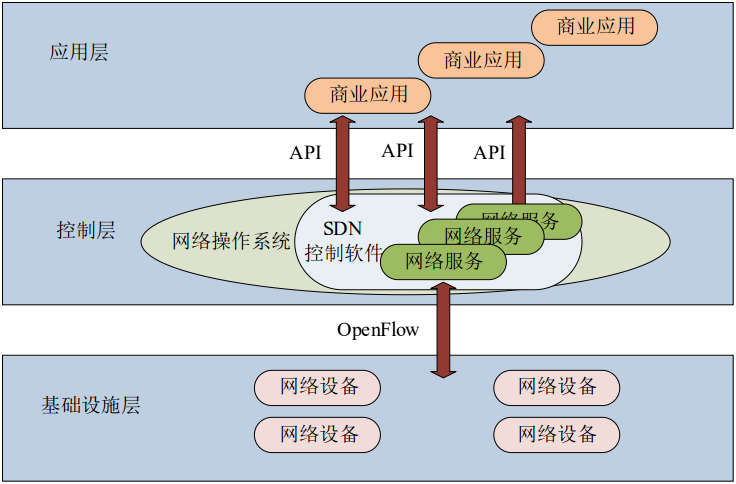
\includegraphics[width=0.7\textwidth]{logo/sdn.png}
  \caption{ONF定义的SDN三层架构图}
  \label{fig:sdn}
\end{figure}

传统网络设备紧耦合的构架在SDN体系中被拆分成应用、控制、转发三层分离的,可编程的开放构架。控制功能被转移到服务器(软件),上层应用、底层转发设施被抽象成多个逻辑实体。图\ref{fig:sdn}为ONF定义的SDN三层架构示意图。

应用层为网络各种应用需求,如移动视频、云存储、企业应用商店、桌面云、物联网等,通过北向接口灵活、可编程地调用控制层提供的网络抽象模型与业务功能。北向接口因为涉及业务较多,开放的标准化过程还处于研究阶段。

控制层为整个SDN构架的核心,也称为网络操作系统,可实现网络拓扑的集中控制和设备管理,进行流表的控制和下发。其主要功能包括路由优化、网络虚拟化、质量监控、拓扑管理、设备管理、接口适配等。

基础设施层包括标准化的网络设备和虚拟的网络设备,负责多级流表处理和高性能的数据转发,并作为硬件资源池,为控制层提供按需的网络拓扑、数据处理和数据转发。目前主流的网络设备和芯片产商已经提供了支持OpenFlow的网络设备。

南向接口定义了控制层与数据转发层(基础设施层)之间的交互协议,通过将转发过程抽象为流表,控制器可直接控制流表、屏蔽硬件,实现了网络虚拟化。物理硬件被淡化为资源池,可按需进行灵活分配和相互隔离。目前主流的控制层与转发层之间交互的协议为OpenFlow协议。
\subsection{OpenFlow协议}
OpenFlow协议是OpenFlow交换机和控制器之间交互信息的标准,也是OpenFlow交换机和控制器之间的接口标准。OpenFlow协议主要支持三种类型的消息:Controller-to-Switch消息,Asynchronous 消息和 Symmetric 消息。每种类型消息都有多个子类型。Controller-to-Switch消息由控制器发起直接管理和监视交换机状态,可能需要交换机做出响应;Asynchronous消息由交换机发起用于更新交换机的状态和控制器的网络事件;Symmetric消息可由控制器和交换机任一方发起。具体协议消息的类型及描述如下:

\begin{enumerate}
\item Controller-to-Switch消息
\begin{itemize}
\item Features:在建立传输层安全会话(Transport Layer Security Session)的时候,控制器发送feature请求消息给交换机,交换机需要应答自身支持的功能。一般在 OpenFlow 通道建立时使用。
\item Configuration:控制器设置或查询交换机上的配置信息。交换机仅需要应答查询消息。
\item Modify-state:控制器管理交换机流表项和端口状态等。
\item Read-state:控制器发送该消息来管理交换机状态。主要用于增加、删除或改变组/流表项和设置交换机端口属性。
\item Packet-out:控制器通过交换机指定端口发出网包。控制器按指定交换机端口发送数据包,并且转发经由Packet-in消息接收到的包。Packet-out消息必须包含完整包或一个指向存储在交换机中的完整包的缓冲区ID。该消息包含一系列按指定顺序执行的行为,若为空则丢弃该包。 
\item Barrier:控制器确保消息依赖满足,或接收完成操作的通知
\end{itemize}
\item Asynchronous消息
\begin{itemize}
\item Packet-in:交换机收到一个网包,在流表中没有匹配项,则发送Packet-in 消息给控制器。如果交换机缓存足够多,网包被临时放在缓存中,网包的部分内容(默认128 字节)和在交换机缓存中的的序号也一同发给控制器;如果交换机缓存不足以存储网包,则将整个网包作为消息的附带内容发给控制器。
\item Flow-removed:交换机中的流表项因为超时或修改等原因被删除掉,会触发Flow-removed 消息,通知控制器删除流表。
\item Port-status:交换机端口状态发生变化时(例如down 掉),触发Port-status 消息。
\item Error:交换机发生问题时触发消息。
\end{itemize}
\item Symmetric消息
\begin{itemize}
\item Hello:交换机和控制器用来建立连接。
\item Echo:交换机和控制器均可以向对方发出Echo消息,接收者则需要回复Echo reply。该消息用来测量延迟、带宽、以及是否连接正常等。
\item Vendor:交换机提供额外的附加信息功能。为未来版本预留。
\end{itemize}
\end{enumerate}

OpenFlow协议的主要交互过程如下所示:

\begin{enumerate}
\item 控制器与交换机的连接建立:通过安全通道建立连接,所有流量都不经过交换机流表检查。当连接建立起来后,两边必须先发送OFPT\_HELLO消息给对方,该消息携带支持的最高协议版本号,接收方将采用双方都支持的最低协议版本进行通信。一旦发现共同支持的协议版本,则连接建立,否则发送OFPT\_ERROR消息,描述失败原因,并中断连接。
\item 控制器与交换机的连接中断:当连接发生异常时,交换机应尝试连接备份的控制器。当多次尝试均失败后,交换机将进入紧急模式,并重置所有的TCP连接。此时,所有包将匹配指定的紧急模式表项,其他所有正常表项将从流表中删除。此外,当交换机刚启动时,默认进入紧急模式。
\item 连接加密:安全通道采用\gls*{TLS}连接加密。当交换机启动时,尝试连接到控制器的TCP 6633端口。双方通过交换证书进行认证。因此,每个交换机至少需配置两个证书,一个是用来认证控制器,一个用来向控制器发出认证。
\item 流表项修改:该交互是核心交互过程,通过控制器下发的流表项修改指令完成。每条指令可能触发一系列OpenFlow协议消息,主要包括流表的增加、修改和删除。
\item 流表项移除:流表项的移出包括控制器主动模式和被动模式,控制器被动模式下,定时器计时结束:每个表项均有一个idle\_timeout定时器和一个hard\_timeout定时器(两者的计量单位都是秒),前者计算的是没有Flow匹配发生的时间,而后者则计算的是表项在流表中的总时间。一旦到达时间期限,交换机将自动删除该表项,同时发出一个流删除的消息;控制器主动模式下,控制器通过下发DELETE\_STRICT、 DELETE等指令相关的协议消息主动删除流表项
\end{enumerate}

\subsection{OpenFlow交换机}
OpenFlow交换机负责数据转发功能,主要技术细节由流表(flow table)、安全信道(secure channel)组成\cite{openflow-1},如图\ref{fig:of-switch}所示。

\begin{figure}[!htb]
  \centering
  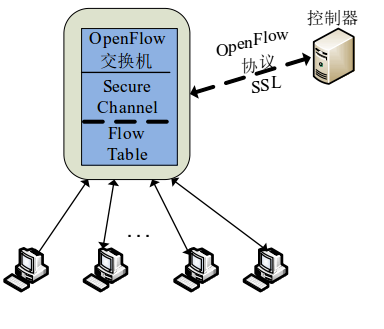
\includegraphics[width=0.7\textwidth]{logo/of-switch.png}
  \caption{OpenFlow交换机结构}
  \label{fig:of-switch}
\end{figure}

OpenFlow的转发策略主要保存在流表中,每个流表中都有很多表项(FlowEntry),这些表项可由外部控制器通过OpenFlow协议来写入、更新和删除。对于OpenFlow\ v1.3,每一个流表项都由匹配域、优先级、计数器、指令、超时以及Cookie组成,如表\ref{table:flow}所示。

\newcommand{\enter}[2][c]{%
  \begin{tabular}[#1]{@{}c@{}}#2\end{tabular}}
\begin{table}[!htb]
    \centering
	\caption{OpenFlow流表项结构}
	\label{table:flow}
	\begin{tabular}{|c|c|c|c|c|c|}
	\hline 
	\enter{匹配域 \\(Match Field)}& \enter{优先级 \\(Priority)}& \enter{计数器 \\(Counters)}& \enter{指令\\(Instructions)}&\enter{超时 \\(Timeouts)} & Cookie \\
	\hline
	\end{tabular}
\end{table}

安全通道是连接OpenFlow交换机和控制器的接口,控制器通过这个接口,按照 OpenFlow协议规定的格式来配置和管理OpenFlow交换机,同时接收交换机传来的事件信息并发送数据包等。所有的OpenFlow通道信息必须用OpenFlow协议打包,OpenFlow通道通常用TLS来加密,但也能直接用TCP协议来实现。

目前,基于软件实现的 OpenFlow交换机主要有两个版本\cite{openflow-2},都部署于 Linux 系统:基于用户空间软件OpenFlow交换机操作简单,便于修改,但性能较差;基于内核空间的软件 OpenFlow 交换机\cite{openflow-3}速度较快,同时提供了虚拟化功能,使得每个虚拟机能够通过多个虚拟网卡传输流量,但实际的修改和操作过程较复杂。另外,斯坦福大学基于 NetFPGA 实现了硬件加速的线速 OpenFlow 交换机\cite{openflow-4},而网络硬件厂商如NEC、HP 等公司也已相继推出了支持 OpenFlow 标准的硬件交换机\cite{openflow-1}。
\subsection{OpenFlow控制器}
\section{网络虚拟化技术概述}
\subsection{传统虚拟化技术及OVX}
\section{OpenStack概述}
\subsection{OpenStack架构}
\subsection{Neutron模块简介}
\section{SDN集成云平台研究现状}
\section{本章小结}


%% 本章参考文献
\ifx\usechapbib\empty
\nocite{BSTcontrol}
\setcounter{NAT@ctr}{0}
\bibliographystyle{buptgraduatethesis}
\bibliography{bare_thesis}
\fi
